\section{Development Methodology}
In order to produce high quality software, a development methodology was selected to monitor, and control all aspects of the project deliverable according to the stakeholder requirements within the expected milestones. 

Six variables were identified that should be managed throughout the project \cite{prince2}. The \textbf{cost} of the project has to be affordable, and need to factor actions that lead to overspending, or opportunities to cut cost. Allied to this, \textbf{time} is the only cost in the project. Ensuring the product delivers on its \textbf{quality}, and is fit for purpose along with the \textbf{scope} where there is an agreement between stakeholders. It is important not to deliver beyond the scope as this is a common source of delays, and uncontrolled change, known as 'scope creep'. Managing the impact of \textbf{risks} is essential, but to assess how much risk there is pivotal. Finally, maintaining the \textbf{benefits} of the stakeholders is of interest so that there is clear understanding of the purpose.

With these factors in mind, the waterfall, agile, and lean methodologies were considered for the project. Waterfall is a fixed sequential framework where it is linear in nature. Each of the eight processes in Waterfall needs to be completed before moving onto the following stage. Despite the easy understanding of the methodology due to strong documentation approaches, this did not suit the project as changes cannot be easily accommodated \cite{smartsheet}. If there were errors during the implementation stage discovered during testing, it would be expensive, and difficult to go back. Further, there is greater reliance over the initial requirements; if these are incorrect they can be detrimental to the project. 

Lean focuses on removing waste from a process in order to deliver products quicker, lowering delivery costs without sacrificing quality, and providing a flexible response to users. This model narrows down to completing the MVP before considering extra features or content, though sometimes the full potential of the project is not reached. Similar to waterfall, the documentation needs to be explicitly precise in the requirements. Further, there were many skills to be acquired by the team throughout the project, and learning on to go is not possible in the lean methodology.

Agile is an iterative, incremental approach that is open to changing requirements with frequent feedback from end users throughout the process. By breaking down the project into small chunks, it makes it easy to prioritise, and add or drop features mid product, which is impossible in traditional waterfall projects. Breaking down tasks into iterations can allow the team to concentrate on high quality implementation. Such an approach delivers measurable results quickly, engages stakeholders earlier, facilitates a more frequent, and reliable product release cycle. However, due to the quick space of the process, the quality of the delivered software could decrease.

With these benefits in Agile, the team decided to adopt this methodology with the scrum framework. Scrum allows for a highly adaptive change in requirements during the entire cycle, and high transparency. The product owner is constantly in touch with the team \cite{globalluxsoft}, and daily stand-up meetings eliminates any misconceptions and confusion. Risk is controlled since issues are identified in advance before getting unmanageable. Kanban was not used since the project required iteration, and prioritising tasks on hand is harder with a Kanban board as all tasks are placed at equal importance with this framework.

\section{Software Development Life Cycle}
In the scrum team, the project supervisor served as the product owner responsible for maximising the value of the product resulting from work of the development team. This ensured the end product delivers value to the end user. The project lead took on the role of scrum master to ensure that stakeholder requirements were met, and to be accountable for the delivery of the sprint goals. The scrum master also took on the role to set and adjust the priorities of the product backlog since they had a greater understanding of the project than the product owner. Having a flat line structure allowed the development team to be self-organising, and cross-functional, with all the skills as a team necessary to create the product increment. According to the framework, scrum recognises no sub-teams in the development team \cite{schwaber}, and this was avoided during implementation. The whole team was accountable for all actions rather than those who have specialised areas of focus. Further, this allowed for dynamic allocation in resources to certain tasks when problems arose.

\begin{figure}[H]
    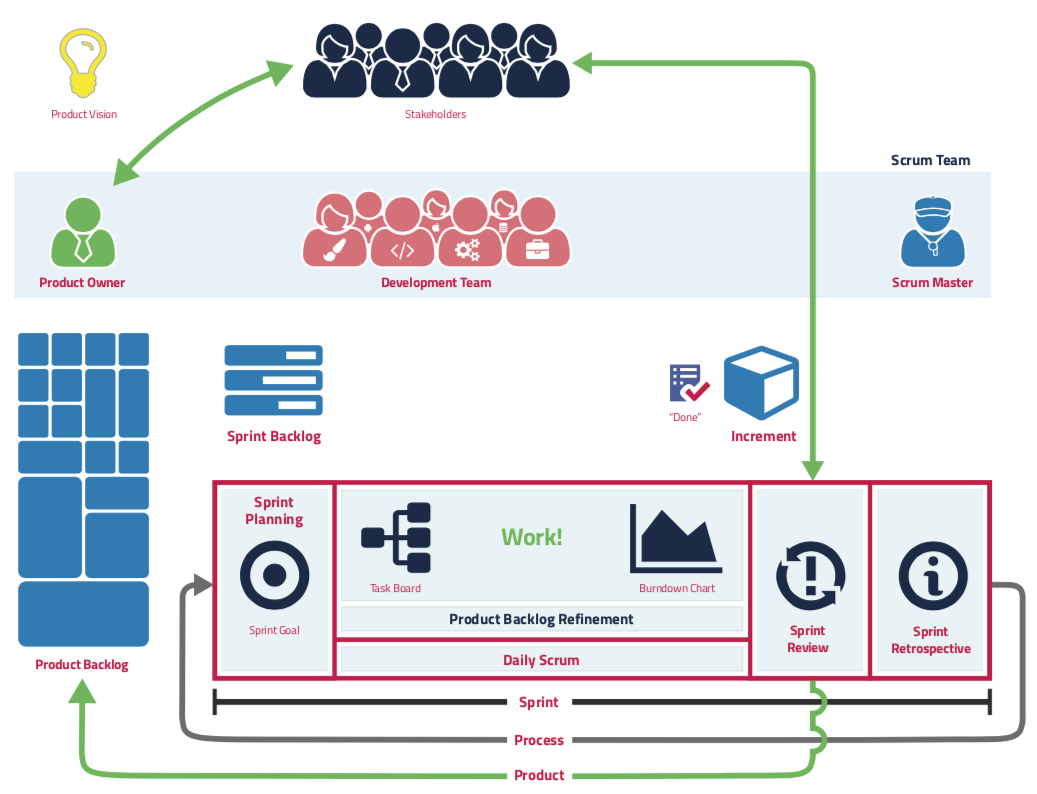
\includegraphics[width=\textwidth, height=100mm]
    {sdlc/scrum.png}
    \caption{The Scrum Workflow \cite{apd}}
    \label{fig:scrumworkflow}
\end{figure}

Scrum events took place such as sprint planning, daily scrum, review, retrospective, and backlog refinement. Sprint planning always took place on the first day of the sprint where three key indicators are outlined, what can get done in the sprint, how the work is done, and the sprint goal \cite{schwaber}, providing the development team an objective. This event usually lasts about one to two hours for a two week sprint. Due to careful planning at the start of every sprint, successful sprints ensued during implementation, and able to deliver on requirements.

Conducting daily scrum proved challenging from the beginning as members were not always on campus at the same time; to resolve this, stand-up would take place at least four times a week. In both terms at the start of every lab, and every supervisor meeting, a ten minute stand-up would happen in person. The other two meetings would happen virtually on Google Hangouts for ten minutes, the day before a milestone deadline (Thursday), and either Saturday or Sunday - depending on the group's availability. Using this model allowed for quick decision-making, and removing any obstacles the team faced.

Sprint reviews took place to audit the work completed, positives, negatives, and problems of the sprint. At this point, the group would decide if the tasks assigned were at "done" status, subject to review of the product owner. All requirements outlined within a reasonable time constraint must be reached to achieve this status. Outstanding tasks to be completed would filter through to the following sprint planning, and the product backlog will be edited accordingly. This formed part of the sprint retrospective, but mainly focused on how well the team administered the methodology. Other key stakeholders are consulted here, giving any important feedback to the completed work.

The team used a scrum board in order to track tasks and make changes during sprints, promoting transparency amongst the group, and ensured accountability was retained. The project used other scrum artifacts discussed in chapter five and six. 

\section{Test-Driven Development}
Another development methodology used was test-driven development (TDD). Before completing implementation for each sprint, unit tests were written so the focus when writing source code is to make all the tests pass. This allows for software architecture to be thought out beforehand, and ensure the core functionality is acting on the requirements. This methodology is proved to reduce defect density, and reduce cost since testing time is dramatically reduced \cite{bulajic}. Further, TDD fits into Agile's iterative approach, providing ease of allocating resources in sprints. Business-driven development, and acceptance test-driven development were considered, but a more thorough and rigorous testing system that focused mainly on the implementation was favored to deliver a working MVP.

\begin{figure}[H]
    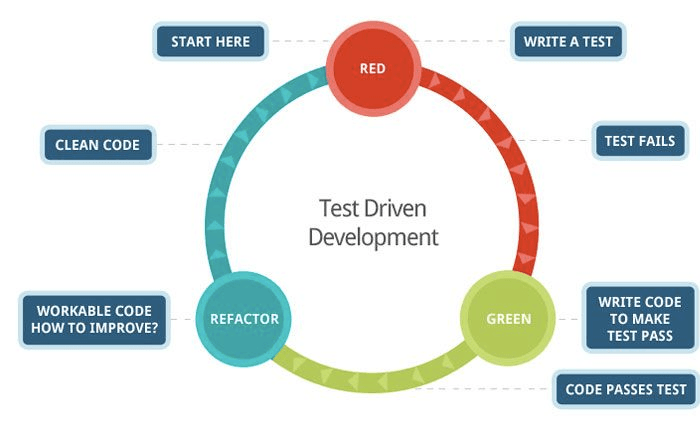
\includegraphics[width=\textwidth]
    {sdlc/tdd.png}
    \caption{The TDD Workflow \cite{k2datascience}}
    \label{fig:tddworkflow}
\end{figure}